\documentclass[crop,tikz]{standalone}% 'crop' is the default for v1.0, before it was 'preview'
%\usetikzlibrary{...}% tikz package already loaded by 'tikz' option
\usepackage{color}
\newcommand{\gv}[1]{\ensuremath{\mbox{\boldmath$ #1 $}}} 
\usepackage{siunitx}

\begin{document}
\fontfamily{cmss}
           {
             \begin{tikzpicture}
               %% \node[label=above:{\Large Starting configuration},label=below:{$\tilde \chi_{\text{AB}}=20$}] (a) at (0,-2) {
               %%   \begin{tikzpicture}

             \node(a) at (0,0) {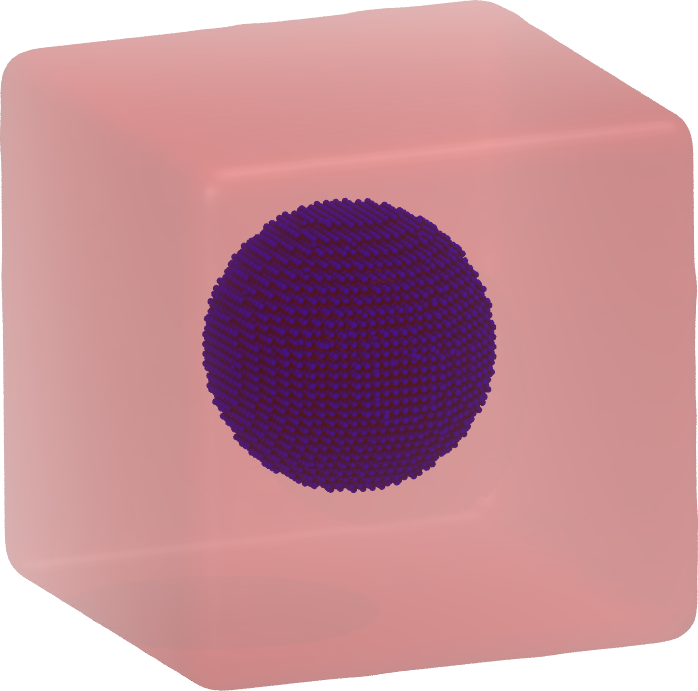
\includegraphics[width=1.5in]{start_sphere.png}};
             \node[fill=white,draw=black,opacity=.7,text opacity=1,rectangle,rounded corners](a2) at([yshift=-.75cm]a.north) {Starting configuration};
             
               %%     \node[rotate=6](b1) at ([xshift=2cm,yshift=0.05cm]a1.south west) {\scriptsize\SI{25}{nm}};
               %%     \node[rotate=-30](b1) at ([xshift=0.4cm,yshift=0.25cm]a1.south west) {\scriptsize\SI{25}{nm}};
               %%     \node[rotate=90](b1) at ([xshift=0.cm,yshift=1.5cm]a1.south west) {\scriptsize\SI{25}{nm}};
               %%   \end{tikzpicture}
               %% };
                
             %[label=below:{$\textcolor{blue}{K_{AB}}=2$}]
             
               \node[](b) at ([yshift=-1.75in]a) {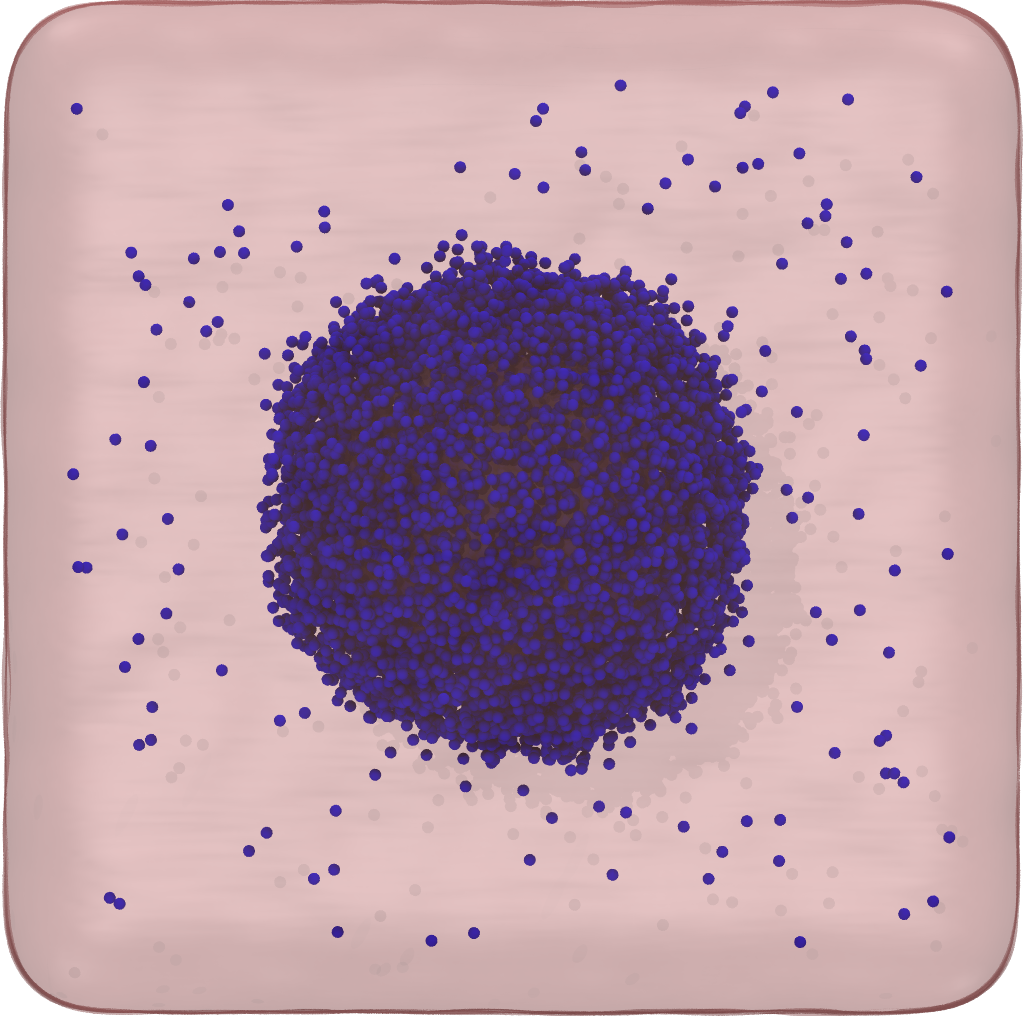
\includegraphics[width=1.5in]{drop5.png}};
               \node[fill=white,draw=black,opacity=.7,text opacity=1,rectangle,rounded corners,anchor=north west]at ([yshift=-0.25cm,xshift=0.25cm]b.north west) {$K_{\text{ST}}=\text{5}$};
               % \draw[->,thick] (a)--node[sloped, anchor=center, above]{$\textcolor{blue}{K_{\text{ST}}}=0$}(b);
               
               \node(c) at ([yshift=-1.75in,xshift=1.75in]a) {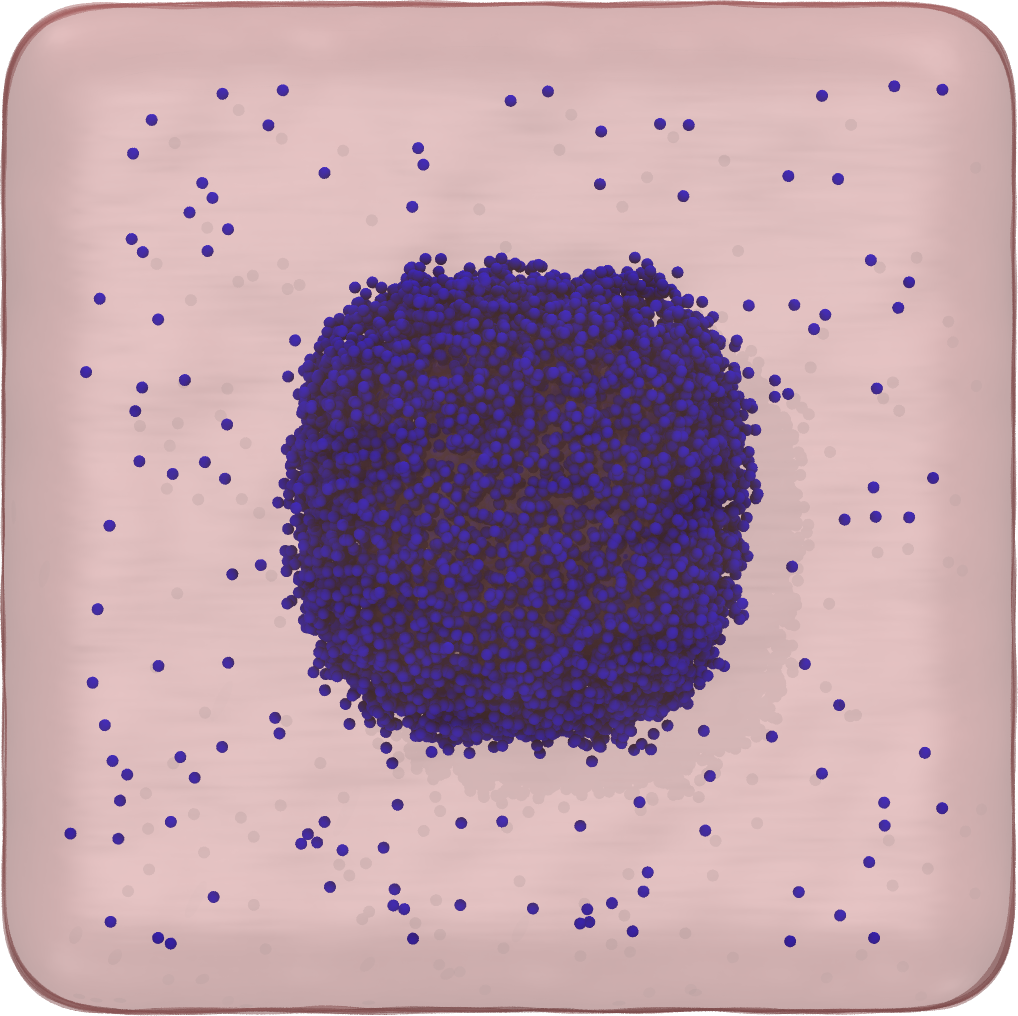
\includegraphics[width=1.5in]{drop0.png}};
               \node[fill=white,draw=black,opacity=.7,text opacity=1,rectangle,rounded corners,anchor=north west]at ([yshift=-0.25cm,xshift=0.25cm]c.north west) {$K_{\text{ST}}=\text{0}$};
               %\draw[->,thick] (a)--node[sloped, anchor=center, above]{$\textcolor{blue}{K_{\text{ST}}}=-5$}(b);

               \node(d) at ([yshift=0,xshift=1.75in]a) {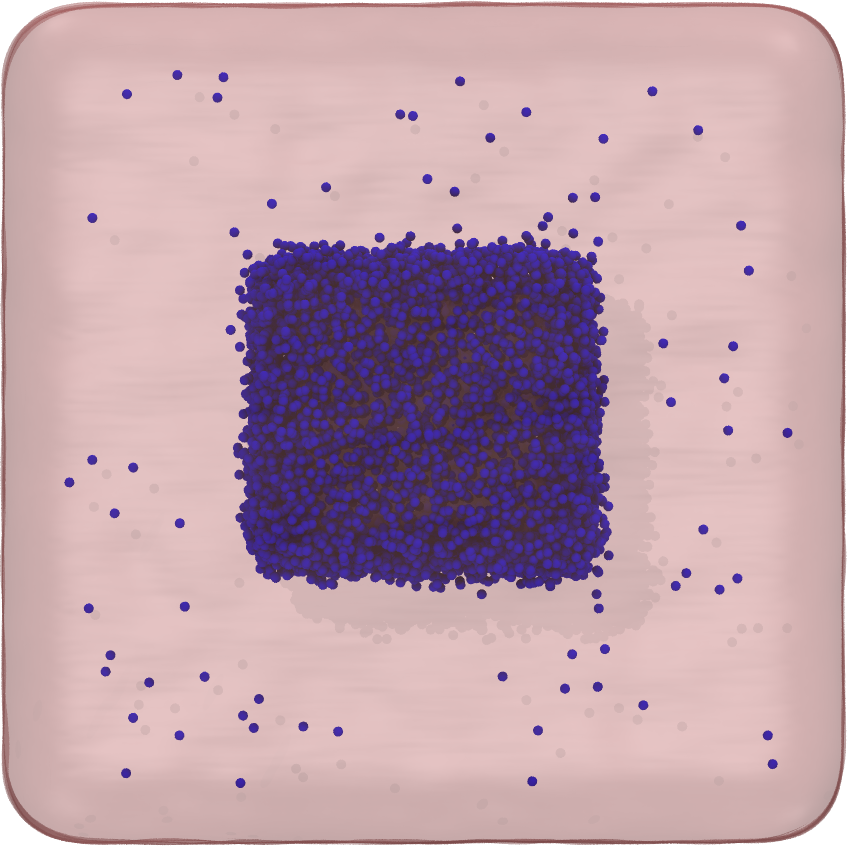
\includegraphics[width=1.5in]{drop-5.png}};
               \node[fill=white,draw=black,opacity=.7,text opacity=1,rectangle,rounded corners,anchor=north west]at ([yshift=-0.25cm,xshift=0.25cm]d.north west) {$K_{\text{ST}}=\text{-5}$};
               %\draw[->,thick] (a)--node[sloped, anchor=center, above]{$\textcolor{blue}{K_{\text{ST}}}=5$}(b);
               
               
               %% \node(e) at (1,-5.25){\(W_1[\gv\nabla\phi]=\frac {-1}{\rho_0}\int\text d \textbf r~  \textcolor{blue}{K_{\text{ST}}}  \gv\nabla\phi_{\text{A}}(\textbf r)\cdot\gv\nabla\phi_{\text{B}}(\textbf r)\)};
               %% \draw[gray,thick,rounded corners]  ([yshift=-0.0cm]e.north west) rectangle ([yshift=-0.cm]e.south east);
             \end{tikzpicture}
           }
\end{document}
